\chapter{Intensity SAR Data}\label{Chapter:DataFormation}

In this chapter we derive the basic properties of SAR data, starting from the complex scattering vector and then reaching the Exponential and Gamma distributions.
With this, we cover what many authors call \textit{fully developed speckle}, or \textit{speckle for textureless targets}.
This will be generalized in Chapter~\ref{Chapter:MultiplicativeModel} for other situations.

Synthetic Aperture Radar (SAR) emits electromagnetic pulses and records the return from the target.
It works in the microwaves region of the spectrum in different bands, as described in Table~\ref{Tab:Bands}.

\begin{table}[hbt]
\caption{SAR Bands (adapted from \url{https://earth.esa.int/handbooks/asar/CNTR5-2.html})}\label{Tab:Bands}
\centering
\begin{tabular}{ccc}
\toprule
\textbf{Band}	& \textbf{Frequency}			& \textbf{Wavelength} \\ \midrule
X-band			& \SIrange[range-units = single]{12.5}{8}{\GHz}	& \SIrange[range-units = single]{2.4}{3.75}{\cm} \\
C-band			& \SIrange[range-units = single]{8}{4}{\GHz} 			& \SIrange[range-units = single]{3.75}{7.5}{\cm}\\
S-band			& \SIrange[range-units = single]{4}{2}{\GHz}	& \SIrange[range-units = single]{7.5}{15}{\cm} \\
L-band			& \SIrange[range-units = single]{2}{1}{\GHz}	& \SIrange[range-units = single]{15}{30}{\cm} \\
P-band			& \SIrange[range-units = single]{0.999}{0.2998}{\GHz}	& \SIrange[range-units = single]{30}{100}{\cm} \\
\bottomrule
\end{tabular}
\end{table}

The frequency, and other parameters such as incidence angle, polarization, and imaging mode, influence the ability of the sensor to retrieve information from the target.
As such, each band is used in a different kind of application:
\begin{description}
\item[X-band:] adequate for high-resolution imaging, as in mapping, agriculture and ocean studies.
\item[C-band:] penetrates tropical clouds and rain showers. Useful in sea ice surveillance and agriculture.
\item[S-band:] rainfall measures and airport surveillance.
\item[L-band:] useful for agriculture, forestry, and soil moisture applications.
\item[P-band:] unaffected by atmospheric effects, significant penetration through vegetation canopies, glacier or sea ice, and soil. Important for estimating vegetation biomass.
\end{description}

Assume we illuminate an area with electromagnetic energy having $N$ elementary backscatterers.
Each backscatterer $i$ will return a fraction of the incident energy $A_i$ with phase $\phi_i$.
The total returned complex signal is, therefore,
\begin{equation}
S = \sum_{i=1}^{N} A_i \exp\{\mathbf j \phi_i\} = 
\underbrace{{\sum_{i=1}^{N} A_i \cos \phi_i}}_{\Re(S)} +\mathbf j \underbrace{ \sum_{i=1}^{N} A_i \sin \phi_i}_{\Im(S)}, 
\label{Eq:ComplexBackscatter}
\end{equation}
where $\mathbf j=\sqrt{-1}$ is the imaginary unit.
This is usually called complex scattering.
Fig.~\ref{Fig:ComplexScattering} illustrates an example with $N=10$ backscatterers (black arrows) and the resulting complex scattering (red arrow).

\begin{marginfigure}
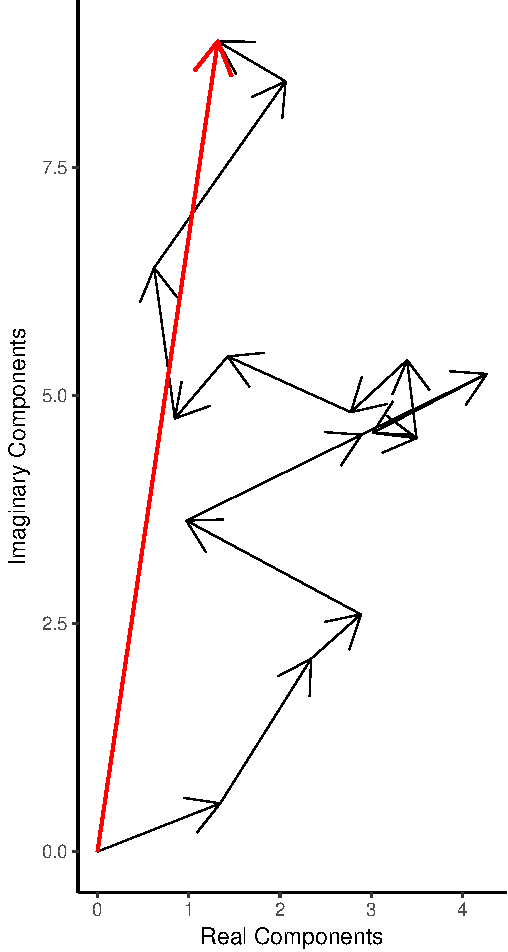
\includegraphics[width=\linewidth]{Scattering}
\caption{Example of complex scattering with $N=10$ elementary backscatterers}\label{Fig:ComplexScattering}
\end{marginfigure}

We have to make some assumptions in order to have a statistical description of the complex return $S$.
First, we are using microwaves whose typical wavelength is of the order of centimeters, and spatial resolutions of the order decimeters.
This leads to the first assumption: $N\to\infty$ if we are observing backscatterers whose size is smaller than the wavelength; think, for instance, of the case of imaging a grass field.
Second, there is no reason to expect that one or a few of these backscatterers dominate the return of the rest; there is no ``mirror'' in our resolution cell.
Third, the (non-negative) amplitudes $A_i$ are independent, with common mean.
Fourth, there is no reason to expect any particular organization or phase dominance; with this, we may assume that the phases $\phi_i$ are outcomes of independent identically distributed Uniform random variables with support $(-\pi,\pi]$.
Fifth, there is no association between phases and amplitudes.

With these hypothesis it is possible to prove that the real and imaginary parts of $S$ are independent Gaussian random variables with zero mean and the same variance $\sigma^2/2$; $\sigma^2$ is often referred to as backscatter.
Two targets with different backscatter only differ in the variance of their complex return $S$.

More often than not, instead of dealing directly with the complex scattering $S$ one prefers to handle its amplitude $A=|S|$ or intensity $I=|S|$.
Without loss of generality, we will prefer the latter.
If the real and imaginary parts of the complex scattering $S$ are independent zero-mean Gaussian random variables with variance $\sigma^2/2$, then the intensity follows an Exponential distribution with mean $\sigma^2$.

A unitary-mean exponential random variable has its distribution characterized by the density
\begin{equation}
f_Z(z) = e^{-z} \mathbb 1_{(0,\mathbb R_+)}(z),
\end{equation}
where $\mathbb 1_{A}(z)$ is the indicator function of the set $A$, i.e., it takes value $1$ inside $A$ and zero otherwise.
Denote this situation $Z\sim E(1)$, and notice that its expected value is $\E(Z)=1$ and its variance is $\Var(Z)=1$.

Being scale-invariant, if $Z'\sim E(1)$, then $Z=\sigma^2 Z'$ has density
\begin{equation}
f_Z(z) = \frac{1}{\sigma^2}e^{-z/\sigma^2} \mathbb 1_{(0,\mathbb R_+)}(z),
\end{equation}
and we denote this situation $Z\sim E(\sigma^2)$.
The cumulative distribution function of $Z\sim E(\sigma^2)$ is 
\begin{equation}
F_Z(z) = (1-e^{-z/\sigma^2}) \mathbb 1_{(0,\mathbb R_+)}(z).
\end{equation}

The mean and variance of $Z\sim E(\sigma^2)$ are, respectively, $\E(Z)=\sigma^2$ and $\Var(Z) = \sigma^4$.
With this, its coefficient of variation is one: $\CV(Z) = \sqrt{\Var(Z)}/\E(Z) = 1$.

Fig.~\ref{Fig:ExponentialDistribution} shows the densities, cumulative distribution functions and densities in semilogarithmic scale of three Exponential distributions, namely those with means equal to $1/2$, $1$ and $2$.

\begin{figure}[hbt]
\centering
\subfloat[Densities]{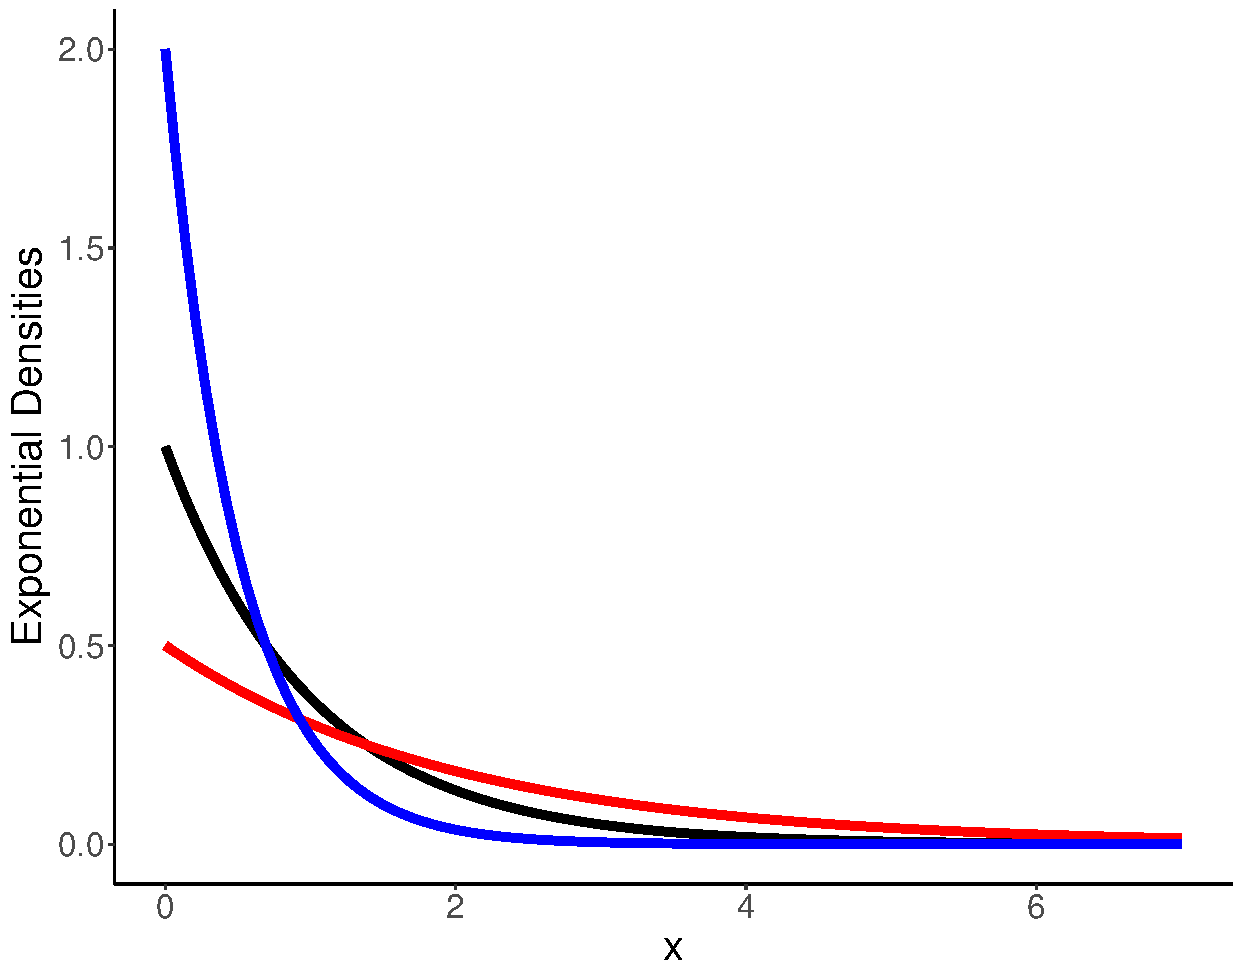
\includegraphics[width=.32\linewidth]{ExponentialDensities}}
\subfloat[Cumulative Distribution Functions]{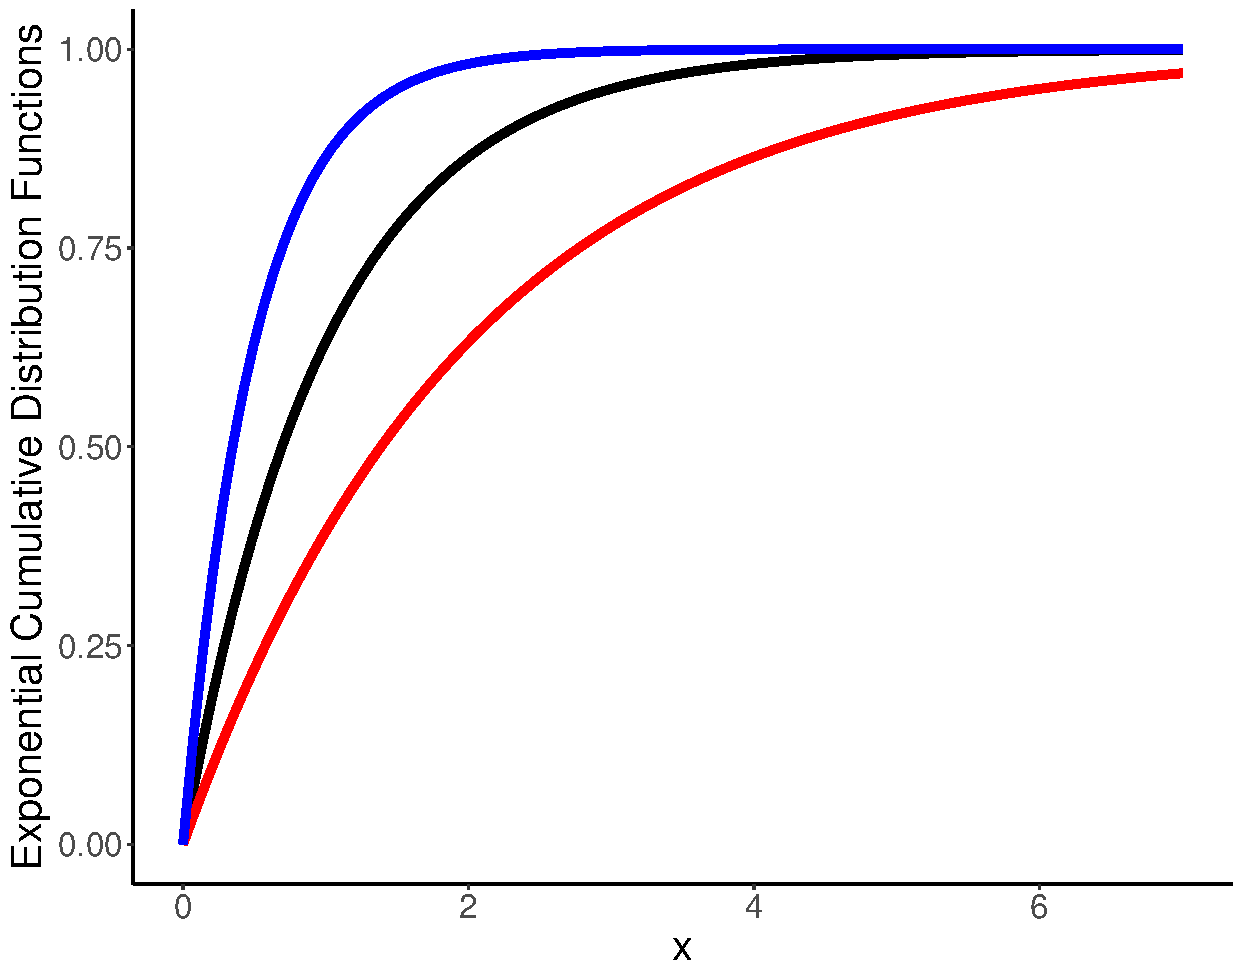
\includegraphics[width=.32\linewidth]{ExponentialCDFs}}
\subfloat[Densities in semilog scale]{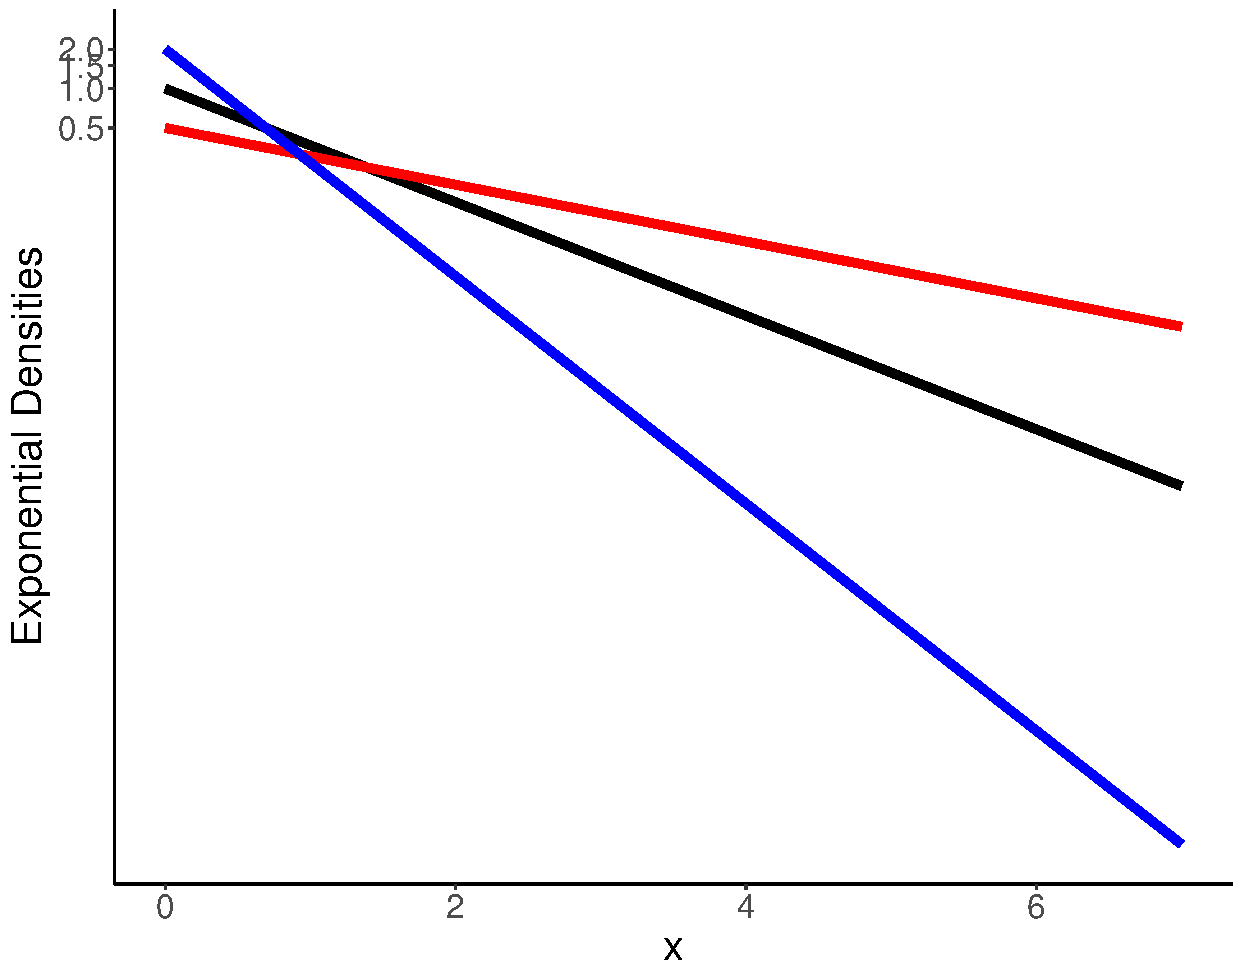
\includegraphics[width=.32\linewidth]{ExponentialDensitiesSemilog}}
\caption{Densities, cumulative distribution functions, and densities in semilogarithmic scale of the exponential distribution with means $1/2$, $1$ and $2$ (red, black, blue, resp.)}\label{Fig:ExponentialDistribution}
\end{figure}

The semilogarithmic scale is particularly useful at revealing the behavior of this distribution for large values: it is linear.

Multilook processing is often applied in order to improve the signal-to-noise ratio, which can be measured as the reciprocal of the coefficient of variation.
It consists of using the mean of $L$ independent observations:
\begin{equation}
Z = \frac1L \sum_{\ell=1}^{L} Z_\ell.
\end{equation}
If each $Z_\ell$ follows an exponential distribution with mean $\sigma^2$, we have that $Z$ obeys a Gamma distribution with mean $\sigma^2$ and shape parameter $L$.
This distribution is characterized by the density
\begin{equation}
f_Z(z;L,\sigma^2) = \frac{L^L}{\sigma^{2L}\Gamma(L)} z^{L-1} 
	\exp\big\{ -L z / \sigma^2
	\big\},
\end{equation}
where $\Gamma(\nu)$ is the Gamma function given by $\Gamma(\nu)=\int_{\mathbb R_+} t^{\nu-1} e^{-t} dt$.
The reader is referred to \citet{abramo-stegu64} for details and relationships with other important special functions.
We denote this situation $Z\sim\Gamma(\sigma^2,L)$
This is also a scale-invariant distribution, in the sense that if $Z'\sim\Gamma(1,L)$, then $Z=\sigma^2 Z'\sim \Gamma(\sigma^2,L)$.

Fig.~\ref{Fig:GammaDistribution} shows three cases of the Gamma distribution with unitary mean and shape parameters (Looks) equal to $1$ (the Exponential distribution), $3$ and $8$.

\begin{figure}[hbt]
\centering
\subfloat[Densities]{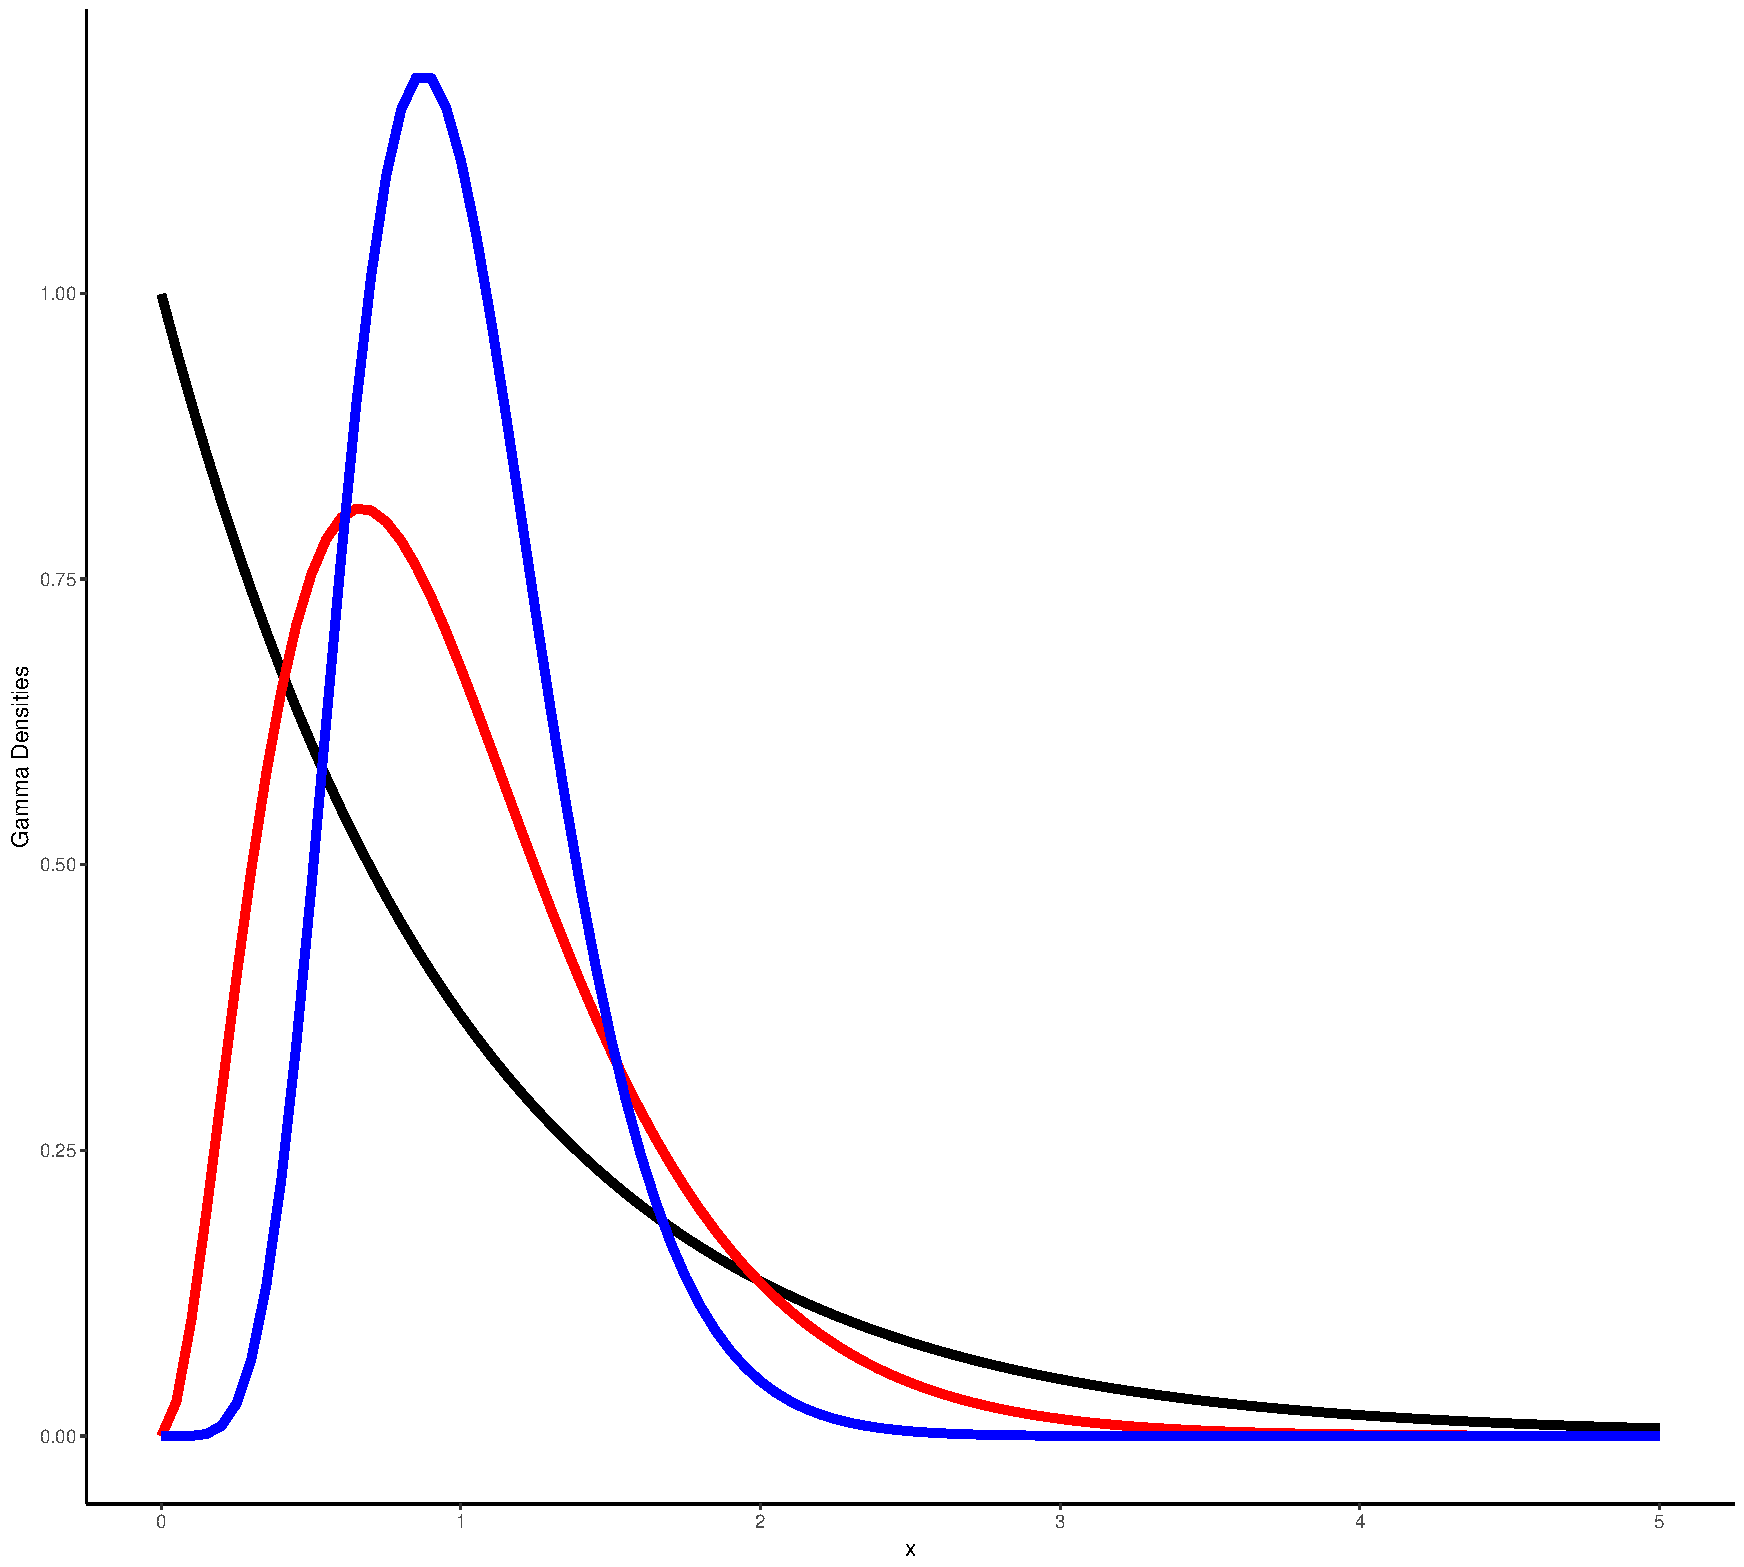
\includegraphics[width=.32\linewidth]{GammaDensities}}
\subfloat[Cumulative Distribution Functions]{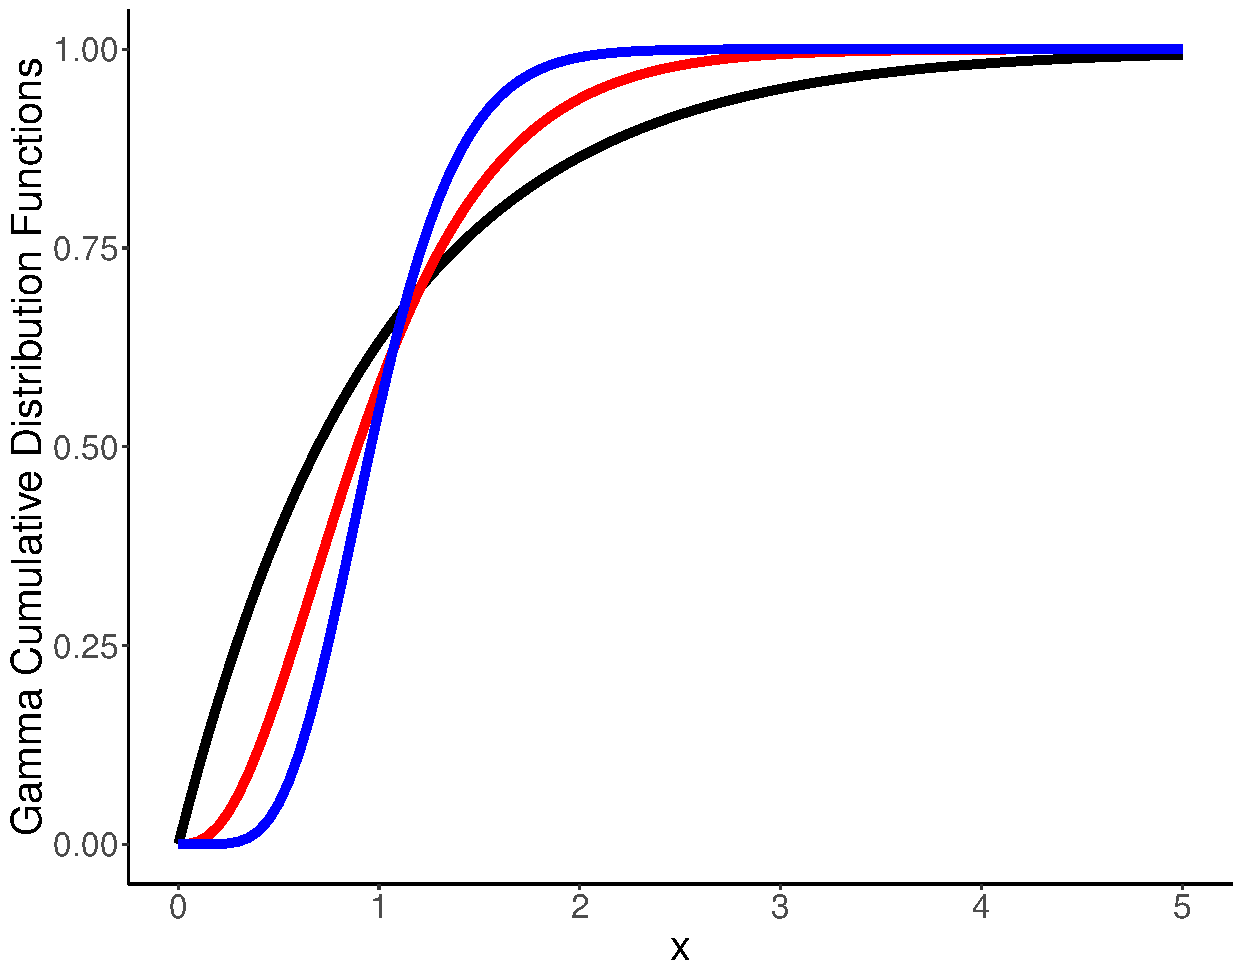
\includegraphics[width=.32\linewidth]{GammaCDFs}}
\subfloat[Densities in semilog scale\label{Fig:DensGammaSemilog}]{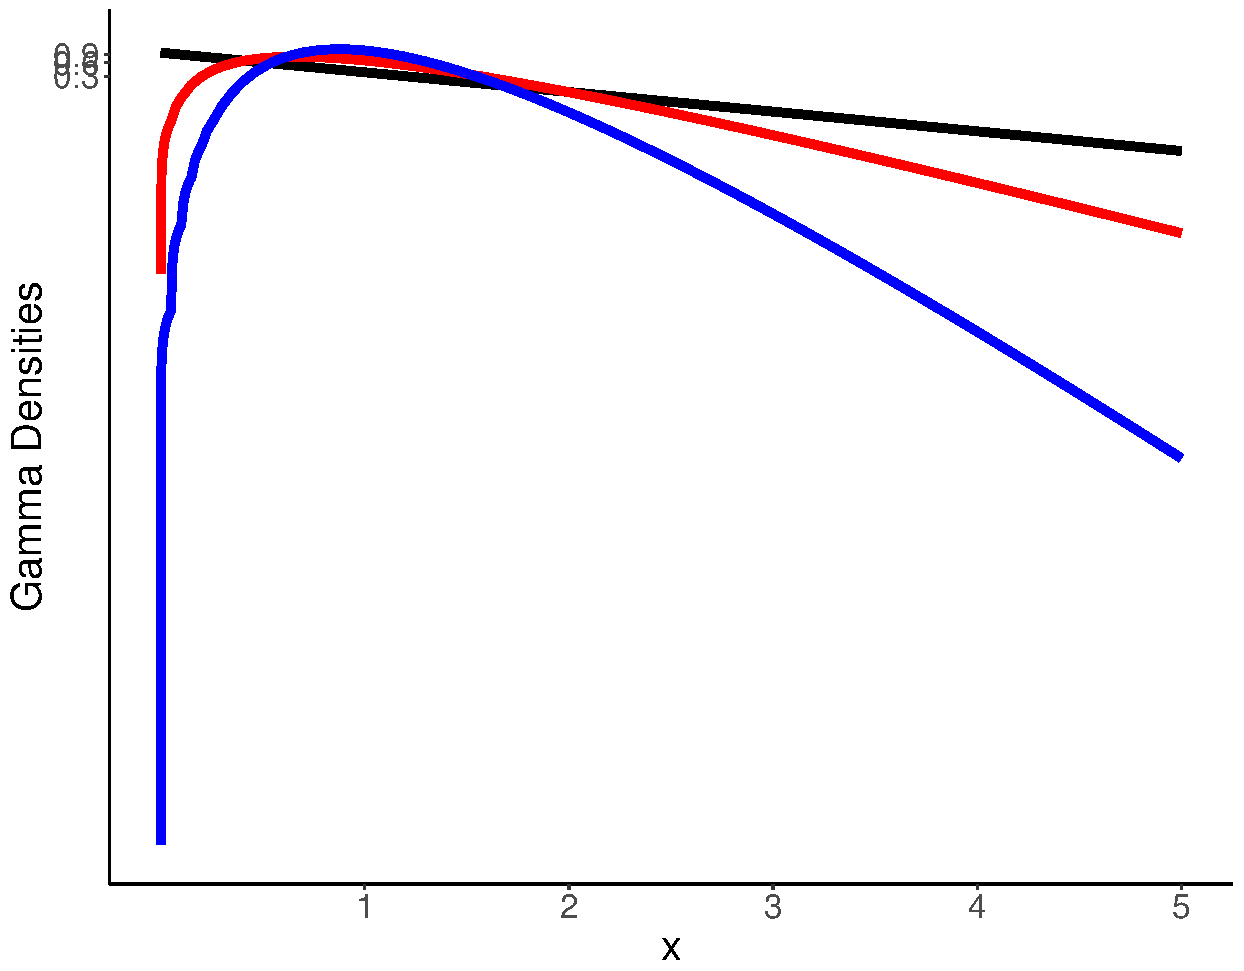
\includegraphics[width=.32\linewidth]{GammaDensitiesSemilog}}
\caption[Densities, cumulative distribution functions, and densities in semilogarithmic scale of the Gamma distribution with unitary mean and shape parameters $1$, $3$ and $8$]{Densities, cumulative distribution functions, and densities in semilogarithmic scale of the Gamma distribution with unitary mean and shape parameters $1$, $3$ and $8$ (red, black, blue, resp.)}\label{Fig:GammaDistribution}
\end{figure}

Fig.~\ref{Fig:GammaDistribution}\subref{Fig:DensGammaSemilog} is important, as this scale shows that the larger the number of looks, the less probable extreme events are.
The Exponential density, being linear

As we mentioned before, the intensity format is not the only possibility.
Assume $Z\sim\Gamma(\sigma^2,L)$ and that $g\colon\mathbb R_+ \to \mathbb R$ is a monotonic function with inverse $g^{-1}$.
The density of the random variable $W = g(Z)$ is given by 
\begin{equation}
f_W(w;L,\sigma^2) = \frac{L^L}{\sigma^{2L}\Gamma(L)} (g^{-1}(w)\big)' \big(g^{-1}(w)\big)^{L-1} 
	\exp\big\{ -L g^{-1}(w) / \sigma^2
	\big\},
	\label{eq:GammmaTransformed}
\end{equation}

Some authors\cite{IterativeWeightedMaximumLikelihoodDenoising} prefer the amplitude format $W=\sqrt{Z}$, while others\cite{Santos2017} opt for a logarithmic transformation $W=\log(Z+1)$ in order to obtain an additive (although not Gaussian) model for the data.
The model for the former is known as \textit{Square Root of Gamma} or \textit{Nakagami} distribution,
while the one for the latter is know as the \textit{Fisher-Tippet} distribution when $L=1$.
The reader is invited to obtain these densities using~\eqref{eq:GammmaTransformed}.

\begin{exer}
Find the densities of the Nakagami and Fisher-Tippet distributions.
Illustrate them.
\end{exer}

\begin{exer}
Assume $Z$ follows a Nakagami distribution.
Find the density of $W=\log(Z+1)$ (a multilook Fisher-Tippet distribution).
Illustrate.
\end{exer}
